\documentclass{book} 
\usepackage[a4paper,left=21mm,right=21mm,top=30mm,bottom=25mm]{geometry}

% general helper packages
\usepackage{amsmath,amsthm}
\usepackage{cancel} 
\usepackage{titlesec}
\usepackage{enumerate} 
\usepackage{fancyhdr}
\usepackage{xfrac}
\usepackage{accents}
\usepackage{stackrel}
\usepackage{nicematrix}
\usepackage{booktabs}

% pretty packages 
\usepackage{graphicx} 
\usepackage[dvipsnames,table]{xcolor}
\usepackage{tikz} 
\usetikzlibrary{automata, arrows.meta, positioning, fit, graphs, quotes}

% pseudocode 
\usepackage[ruled, linesnumbered,vlined]{algorithm2e}
\SetArgSty{}

% fonts 
\usepackage{classico} % sans serif font
\usepackage{inconsolata} % typewriter font
\usepackage{newpxtext} % text font
\usepackage[euler-digits]{eulervm} % math font
\usepackage[bb=stixtwo]{mathalpha} % bb alphabet

% nicer math symbols for subset, union/intersection, etc.
\DeclareFontFamily{U}{matha}{\hyphenchar\font45}
\DeclareFontShape{U}{matha}{m}{n}{
      <5> <6> <7> <8> <9> <10> gen * matha
      <10.95> matha10 <12> <14.4> <17.28> <20.74> <24.88> matha12
      }{}
\DeclareSymbolFont{matha}{U}{matha}{m}{n}
\DeclareFontSubstitution{U}{matha}{m}{n}

\DeclareMathSymbol{\subseteq}{3}{matha}{"84}
\DeclareMathSymbol{\subset}{3}{matha}{"80}
\DeclareMathSymbol{\nsubset}{3}{matha}{"86}
\DeclareMathSymbol{\in}{3}{matha}{"50}
\DeclareMathSymbol{\nin}{3}{matha}{"52}
\DeclareMathSymbol{\cup}{3}{matha}{"59}
\DeclareMathSymbol{\cap}{3}{matha}{"58}
\DeclareMathSymbol{\complement}{3}{matha}{"41}
\DeclareMathSymbol{\to}{3}{matha}{"D1}
\DeclareMathSymbol{\gets}{3}{matha}{"D0}

\usepackage[hidelinks]{hyperref}
\usepackage{setspace}
\usepackage{mdframed}

\title{math62.1 lec notes} 
\author{emily} 
\date{\today}

\pagestyle{fancy}
\fancyhead{}
\fancyhead[LE]{\nouppercase\leftmark}% LE -> Left part on Even pages
\fancyhead[RO]{\nouppercase\rightmark}% RO -> Right part on Odd pages

\RenewDocumentCommand{\labelitemi}{}{$\rightarrow$}
\RenewDocumentCommand{\labelenumi}{}{\colorbox{Periwinkle!40}{\textbf{\arabic{enumi}}}}
\RenewDocumentCommand{\labelenumii}{}{\transparent{0.5}\colorbox{CornflowerBlue!40}{\transparent{1.0}\textbf{\alph{enumii}}}}

\NewDocumentEnvironment{solution}{}{%
    \RenewDocumentCommand{\qedsymbol}{}{$\blacksquare$}
    \begin{proof}[Solution]
}{\end{proof}}

\NewDocumentEnvironment{example}{}{
    \RenewDocumentCommand{\qedsymbol}{}{$\blacksquare$}
    \begin{proof}[Example]
}{\end{proof}}

\newcounter{theo}[section]


\newenvironment{theorem}[1][]{%
  \refstepcounter{theo}%
  \ifstrempty{#1}%
    {\mdfsetup{%
      frametitle={%
        \tikz[baseline=(current bounding box.east),outer sep=0pt]
        \node[anchor=east,rectangle,fill=Periwinkle!40]
        {\strut{}\textsf{Theorem~\thesection.\thetheo}};}}
    }%
    {\mdfsetup{%
frametitle={%
\tikz[baseline=(current bounding box.east),outer sep=0pt]
\node[anchor=east,rectangle,fill=Periwinkle!40]
{\strut\textsf{Theorem~\thesection.\thetheo:~#1}};}}%
}%
\mdfsetup{innertopmargin=2pt,linecolor=Periwinkle!40,%
linewidth=2pt,topline=true,
frametitleaboveskip=\dimexpr-\ht\strutbox\relax,}
\begin{mdframed}[]\relax%
}{\end{mdframed}}

\titleformat{\chapter}[block]
  {\normalfont\LARGE\bfseries}{\colorbox{Periwinkle!40}{\sffamily\thechapter}}{1em}{\LARGE\sffamily}
\titlespacing*{\chapter}{0pt}{-19pt}{10pt}

\titleformat{\section}{\bfseries}{\Large\sffamily\thechapter.\arabic{section}}{1em}{\Large\sffamily
\RenewDocumentCommand{\labelenumi}{}{\colorbox{magenta!40}{\textbf{\arabic{enumi}}}}}

\NewDocumentCommand{\exercises}{}{\vspace{10pt}\noindent\textbf{\large Exercises}}

\NewDocumentCommand{\prop}{}{\noindent\refstepcounter{theo}\textbf{\textsf{Proposition~\thesection.\thetheo.}}}
\NewDocumentCommand{\lemm}{}{\noindent\refstepcounter{theo}\textbf{\textsf{Lemma~\thesection.\thetheo.}}}
\NewDocumentCommand{\cor}{}{\noindent\refstepcounter{theo}\textbf{\sffamily{}Corollary \thesection.\thetheo.}}
\NewDocumentCommand{\exm}{}{\noindent\refstepcounter{theo}\textbf{\sffamily{}Example \thesection.\thetheo.}}
\NewDocumentCommand{\rem}{}{\noindent\textbf{\sffamily{}Remark.}}

\onehalfspacing\setlength{\parskip}{5pt}


\NewDocumentCommand{\lang}{}{\mathsf{L}}
\NewDocumentCommand{\machine}{}{\mathsf{M}}
\NewDocumentCommand{\endex}{}{
  \begingroup
  \RenewDocumentCommand{\qedsymbol}{}{\(\bullet\)}
  \qed\endgroup}

\begin{document}

\setcounter{chapter}{-1}
\chapter{Preliminaries}\label{ch:intro}
The study of finite automata originally began with theoretical linguists in the mid 20th century trying to understand how language works. 
They wanted to fully capture the process of language making through a series of formal rules and automatic methods---hence, creating machines that could mimic language ``perfectly''. 
They failed, obviously, because language is constantly evolving and can't be tied down by a fixed set of rules. 
However, a lot of their theory became useful in the study of \emph{formal languages} (e.g., programming languages), where the rules are fixed by design in order to avoid unwanted behaviour in machines. 
This is why a lot of the terminology uses words like `alphabets' and `languages'. 
In this section, we fix a few terms and review some set-theoretic concepts. 

\section{Strings, languages, and decision problems} 

An \emph{alphabet} \(\Sigma\) is a finite, non-empty set of symbols. 
A \emph{string} \(w = a_1 a_2 \cdots a_k\) of length \(k\) is a sequence of \(k\) symbols \(a_i \in \Sigma\). 
We write \(|w| = k\) to indicate that the string has length \(k\). 
We also define for convenience the empty word, \(\varepsilon\), which has length \(0\). 

\exm{} For example, given the binary alphabet \(\Sigma = \{0,1\}\), \(001\) is a word of length \(3\).\endex{}

We define \(\Sigma^k\) to be the set of all \(k\)-length words from the alphabet. 
By convention, \(\Sigma^0 = \{ \varepsilon \}\). 

\exm{} Taking the binary alphabet \(\Sigma = \{0, 1\}\) again, we have\[
    \Sigma^k = \{ 000, 001, 010, 011, 100, 101, 110, 111 \},
\]for example.\endex{}

The \emph{Kleene closure} of an alphabet is defined as\[    
\Sigma^* = \Sigma^0 \cup \Sigma^1 \cup \Sigma^2 \cup \cdots \]
We also define \(\Sigma^+ = \Sigma^1 \cup \Sigma^2 \cup \cdots\). 
Intuitively \(\Sigma^*\) is the set of all possible finite strings given characters from that alphabet, along with the empty string. 
Note that \(\Sigma^*\) is always infinite. 

\exm{} For example, the set \(\Sigma^*\) over the binary alphabet is the set of all allowable binary strings, plus the empty word:\[
    \Sigma^* = \{\varepsilon, 0, 1, 00, 01, 10, 11, 000, 001, 010, 011, \ldots \}
\]\endex{}

\emph{Concatentation} of strings is defined in an obvious way: given two strings \(w_1\) and \(w_2\), concatenating them results in \(w_1 w_2\). 
Concatenating any string with \(\varepsilon\) results in the same string. 
Similarly, a word \(w_1\) is a \emph{prefix} of \(w\) if \(w = w_1 w_2\), and a \emph{suffix} of \(w\) if \(w = w_2 w_1\). We write\[
w^k = \underbrace{ww\cdots w}_{k~\text{times}}
\]and if \(w = a_1 a_2 \cdots a_k\) for \(a_i \in \Sigma\), then \(w^\mathrm{R} = a_k a_{k-1} \cdots a_1\) is the reverse of \(w\). 
We also define \emph{substrings} in an obvious way. A string \(s\) is a substring of \(w\) if there exist (possibly empty) strings \(u, v\) such that \(w = usv\). 

A \emph{language} \(\mathsf{L}\) over an alphabet \(\Sigma\) is any set of words over \(\Sigma\), i.e., a subset \(\mathsf{L} \subseteq \Sigma^*\). 
Since languages are sets, we can define the usual set operations of union, intersection, complement, and set difference on them. 
We also define some language-specific operations: the concatenation of two languages,\[
\mathsf{L}_1 \mathsf{L}_2 = \{w_1 w_2 \mid w_1 \in \mathsf{L}_1~\text{and}~w_2 \in \mathsf{L}_2\},~\text{with}~\mathsf{L}_1^k = \underbrace{L_1 L_1 \cdots L_1}_{k~\text{times}}, 
\]and \(L_1^0 = \{\varepsilon\}\) as usual; and the Kleene closure of a language, \[
\lang^* = \lang^0 \cup \lang^1 \cup \lang^2 \cup \cdots
\]

\exm{} For a simple example, take the languages \(\lang_1 = \{00, 11\}\) and \(\lang_2 = \{01, 10\}\). We then have \[
\lang_1 \lang_2 = \{0001, 0010, 1101, 1110\},~\lang_2 \lang_1 = \{0100, 0111, 1000, 1011\}.
\]Notice that concatenation is not in general commutative. We also have\[
\lang_1^* = \{\varepsilon, 00, 11, 0000, 0011, 1100, 1111, 000000, 000011, 001100, \ldots \}.\]\endex{}

Beyond applications in programming language design, these languages are useful to us because we can represent the solutions of a certain problem with a certain language. 
For instance, if a given problem is to determine whether or not a binary number is divisible by three, then an equivalent ``solution'' to that problem would be the set of all binary strings that are divisible by three, along with a process of determining whether or not an arbitrary string belongs to this language. 
This process of determining whether or not a string is contained inside a language is called a \emph{decision problem}. 

\section{A little bit of set theory}

\section{Notes on proofs} 

There will be proving in this class, but the arguments we use will generally be \textit{constructive}. 
\chapter{Deterministic finite automata and regular languages}
In this chapter, we will cover models of computation that all correspond to (spoilers!) one kind of language: that of the \emph{regular languages}. 
This will be the weakest form of computation we will consider in this course, but a lot of the same ideas will be present throughout later chapters, so this is a good starting point to gain experience dealing with machines and languages in general. 
For an overview, we begin by introducing the deterministic finite automata and the kind of languages they compute. 
Then, we will attempt to prove that these languages are \emph{closed} under certain operations, which will lead us to two new kinds of automata: \emph{non}deterministic FAs and so-called \(\varepsilon\)-nondeterministic FAs. 
We will show that these two models of computation, though seemingly more powerful than the DFAs, actually capture the same kinds of languages. 
Finally, we will create languages that \emph{cannot} be captured by any DFA, using a powerful result known as the pumping lemma. 

\section{DFAs}
The first model of computation we will tackle is that of a \emph{deterministic finite automaton}, or \emph{DFA}. 
DFAs consist of finitely many states which are either accepting or not, and we model computation as the DFA taking in \emph{input strings} and moving to a new state at each step of the computation depending on the currently read symbol and the current state the machine is in. 
Certain states of the DFA will be marked as \emph{accepting} states, so that if the computation given an input string terminates in an accepting state, we say that the string is \emph{accepted} by the DFA. 
The set of all strings accepted by the DFA is its language. 

DFAs being \emph{deterministic} means that there is exactly one way to compute given an input string. 
It also means that given a state and given a symbol, there will always be a next state to go to; in terms that we will learn later on, this means that the \emph{transition function} is complete over the set of inputs. 
In general, we will only consider DFAs over the alphabet \(\Sigma = \{0, 1\}\). 

\exm{} Let \(\lang_1 = \{ w\in\Sigma^* \mid 00~\text{is a substring of}~w\} \). Thus, \(\lang_1 = \{ 00, 001, 100, 000, 1000, 1001, \ldots \} \). 
The DFA that accepts this language is given by:\begin{center}
    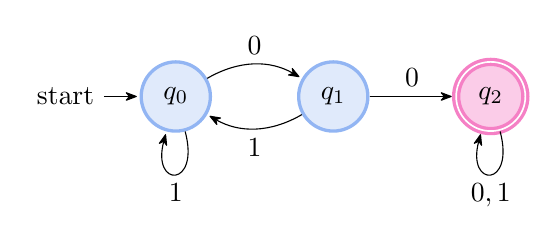
\begin{tikzpicture}[shorten >=1pt,node distance=2cm,on grid,>={Stealth[round]},
        every state/.style={draw=CornflowerBlue!70,fill=CornflowerBlue!20,very thick}, 
        accepting/.style={draw=magenta!50,fill=magenta!20, very thick,double}]
    
      \node[state,initial]  (q_0)                      {$q_0$};
      \node[state]          (q_1) [right=of q_0] {$q_1$};
      \node[state, accepting]          (q_2) [right=of q_1] {$q_2$};
    
      \path[->] (q_0) edge [bend left]             node[above]  {\(0\)} (q_1)
                      edge [loop below]             node  {\(1\)} ()
                (q_1) edge node[above]           {\(0\)} (q_2)
                edge [bend left] node[below] {\(1\)} (q_0) 
                (q_2) edge [loop below] node               {\(0,1\)} ();
    \end{tikzpicture}
\end{center}
In this diagram, we start the computation at the indicated starting state, and the accepting states are marked with a double outline and a different color. 
Let's go through the process of accepting a string, \(1001\). 
\begin{center}
    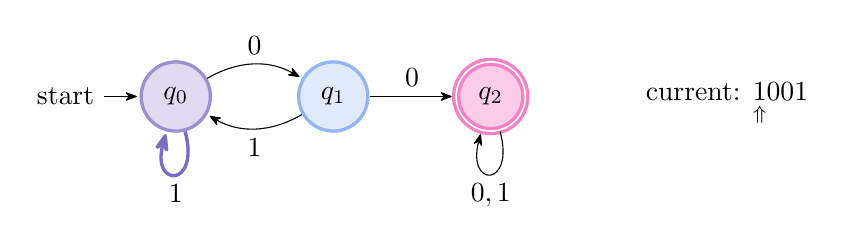
\begin{tikzpicture}[shorten >=1pt,node distance=2cm,on grid,>={Stealth[round]},
        every state/.style={draw=CornflowerBlue!70, fill=CornflowerBlue!20,very thick}, 
        accepting/.style={draw=magenta!50,fill=magenta!20, very thick,double}]
        % \draw[help lines] (-1,-1) grid (8,1);
    
      \node[state,initial,draw=Periwinkle!70, fill=Periwinkle!20]  (q_0)                      {$q_0$};
      \node[state]          (q_1) [right=of q_0] {$q_1$};
      \node[state, accepting]          (q_2) [right=of q_1] {$q_2$};
      \node (word) at (7,-0.1)  {current: \(\underset{\Uparrow}{1}001\)};
    
      \path[->] (q_0) edge [bend left]             node[above]  {\(0\)} (q_1)
                      edge [loop below,very thick,draw=Periwinkle]             node  {\(1\)} ()
                (q_1) edge node[above]           {\(0\)} (q_2)
                edge [bend left] node[below] {\(1\)} (q_0) 
                (q_2) edge [loop below] node               {\(0,1\)} ();
    \end{tikzpicture}
\end{center}
We begin at state \(q_0\), reading the symbol \(1\). 
The arrow coming out of the state labelled with a \(1\) instructs us to stay in state \(q_0\) when reading that symbol, so we ``consume'' that symbol and move to the next. 
\begin{center}
    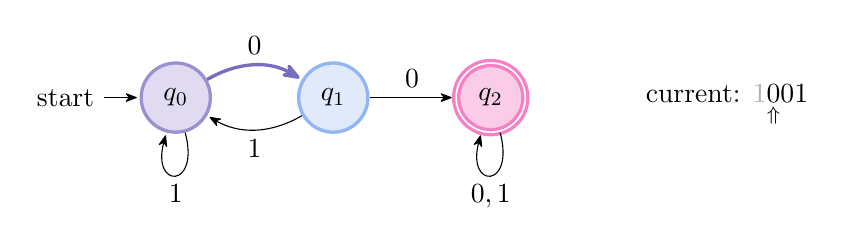
\begin{tikzpicture}[shorten >=1pt,node distance=2cm,on grid,>={Stealth[round]},
        every state/.style={draw=CornflowerBlue!70,fill=CornflowerBlue!20,very thick}, 
        accepting/.style={draw=magenta!50,fill=magenta!20, very thick,double},]
    
      \node[state,initial, draw=Periwinkle!70,fill=Periwinkle!20]  (q_0)                      {$q_0$};
      \node[state]          (q_1) [right=of q_0] {$q_1$};
      \node[state, accepting]          (q_2) [right=of q_1] {$q_2$};
      \node (word) at (7,-0.1)  {current: \(\textcolor{black!30}{1}\underset{\Uparrow}{0}01\)};
    
      \path[->] (q_0) edge [bend left,very thick,draw=Periwinkle]             node[above]  {\(0\)} (q_1)
                      edge [loop below]             node  {\(1\)} ()
                (q_1) edge node[above]           {\(0\)} (q_2)
                edge [bend left] node[below] {\(1\)} (q_0) 
                (q_2) edge [loop below] node               {\(0,1\)} ();
    \end{tikzpicture}
\end{center}
Now we are in state \(q_0\), reading the symbol \(0\). 
The arrow coming out of the state labelled with a \(0\) instructs us to move to state \(q_1\), so again we consume the \(0\) and move on. 
\begin{center}
    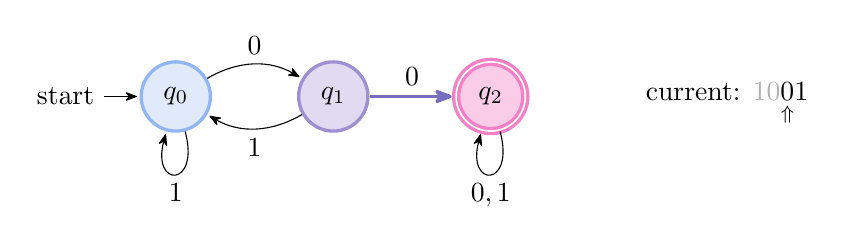
\begin{tikzpicture}[shorten >=1pt,node distance=2cm,on grid,>={Stealth[round]},
        every state/.style={draw=CornflowerBlue!70,fill=CornflowerBlue!20, very thick}, 
        accepting/.style={draw=magenta!50,fill=magenta!20, very thick,double}]
    
      \node[state,initial]  (q_0)                      {$q_0$};
      \node[state, draw=Periwinkle!70, fill=Periwinkle!20]          (q_1) [right=of q_0] {$q_1$};
      \node[state, accepting]          (q_2) [right=of q_1] {$q_2$};
      \node (word) at (7,-0.1)  {current: \(\textcolor{black!30}{10}\underset{\Uparrow}{0}1\)};
    
      \path[->] (q_0) edge [bend left]             node[above]  {\(0\)} (q_1)
                      edge [loop below]             node  {\(1\)} ()
                (q_1) edge [very thick,draw=Periwinkle] node[above]           {\(0\)} (q_2)
                edge [bend left] node[below] {\(1\)} (q_0) 
                (q_2) edge [loop below] node               {\(0,1\)} ();
    \end{tikzpicture}
\end{center}
Now we are in state \(q_1\), reading the symbol \(0\). 
The arrows instruct us to move to state \(q_2\) and consume the \(0\). 
\begin{center}
    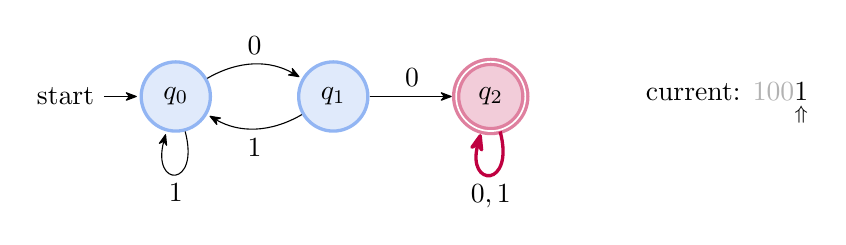
\begin{tikzpicture}[shorten >=1pt,node distance=2cm,on grid,>={Stealth[round]},
        every state/.style={draw=CornflowerBlue!70,fill=CornflowerBlue!20, very thick}, 
        accepting/.style={draw=purple!50,fill=purple!20, very thick,double}]
    
      \node[state,initial]  (q_0)                      {$q_0$};
      \node[state]          (q_1) [right=of q_0] {$q_1$};
      \node[state, accepting]          (q_2) [right=of q_1] {$q_2$};
      \node (word) at (7,-0.1)  {current: \(\textcolor{black!30}{100}\underset{\Uparrow}{1}\)};
    
      \path[->] (q_0) edge [bend left]             node[above]  {\(0\)} (q_1)
                      edge [loop below]             node  {\(1\)} ()
                (q_1) edge node[above]           {\(0\)} (q_2)
                edge [bend left] node[below] {\(1\)} (q_0) 
                (q_2) edge [loop below,very thick, draw=purple] node               {\(0,1\)} ();
    \end{tikzpicture}
\end{center}
Now, we have just a \(1\) left, and the arrows instruct us to stay in place once again. 
This leaves us with no more symbols to read, which means that the computation has ended. 
As we can also see, the computation finished in an accepting state, so the string will be accepted. 
If we repeat the procedure for a string without any \(00\) contained in it, like \(1101\), we will see that the computation never reaches beyond state \(q_1\). 
Try it out!\endex{}

Keeping this example in mind, we can now give the formal definition of a DFA: a deterministic finite automaton \(\machine\) consists of the following data:\begin{enumerate}
    \item a finite set \(Q = \{q_0, q_1, \ldots, q_n \} \) of \emph{states}; 
    \item an alphabet of allowed symbols \(\Sigma\); 
    \item a \emph{transition function} \(\delta : Q \times \Sigma \to Q\), which takes in as input a state and a symbol from the alphabet, and returns a (possibly different) state; 
    \item an \emph{initial} or \emph{starting state} \(q_0\); and 
    \item a subset \(F\subseteq Q\) of states known as \emph{final} or \emph{accepting states}. 
\end{enumerate}
We may represent this data by writing \(\machine = \langle Q, \Sigma, \delta, q_0, F \rangle\) when we specify a certain DFA. 

\exm{} With the same DFA as the last example, we can see that \(Q = \{q_0, q_1, q_2\}\), \(\Sigma = \{0, 1\}\), the transition function \(\delta\) is given by the diagram, \(q_0\) is the initial state, and \(F = \{q_2 \}\). 
We may also specify a transition function by a complete table of possible inputs and outputs. 
If we also highlight the starting states and accepting states, then the table conveys the exact same information as the diagram above:\begin{center}
    \begin{tabular}{c|cc}
        \toprule
        state & \(0\) & \(1\) \\ 
        \midrule
        \(\to q_0\) & \(q_1\) & \(q_0\) \\ 
        \(q_1\) & \(q_2 \) & \(q_0\) \\ 
        \(q_2 \to\) & \(q_2\) & \(q_2\) \\
        \bottomrule
    \end{tabular}
\end{center}
Here, we signified the starting states by an arrow coming in, and the final states by an arrow coming out.
In general, we may use either representation, depending on which is more convenient---though admittedly, I prefer using the diagrams because they're prettier! \endex{}

\vspace{10pt}
\begin{minipage}{.14\textwidth}
    \includegraphics[width=2cm]{nerd_maddy.png} 
\end{minipage}%
\fcolorbox{Periwinkle}{white!100}{
\begin{minipage}{.76\textwidth}
    \textbf{Nerd Interjection!} It's good practice to give meaning to our states, i.e., try to figure out what being in a certain state means. 
    In the previous DFA, we move to \(q_1\) upon reading a \(0\), but we are only sure that there are two consecutive \(0\)'s if we read another \(0\) while in \(q_1\). 
    If we read a \(1\) instead, we go back to \(q_0\). 
    Thus, \(q_1\) is a state of ``expecting'' another \(0\). 
    Of course, this machine is not really expecting anything, being incapable of thought. 
\end{minipage}}
\vspace{10pt}

\exm{} Consider the language \(\lang_1 = \{ w \in \Sigma^* \mid 00~\text{is a suffix of}~w \}\). 
A DFA for this language is:\begin{center}
    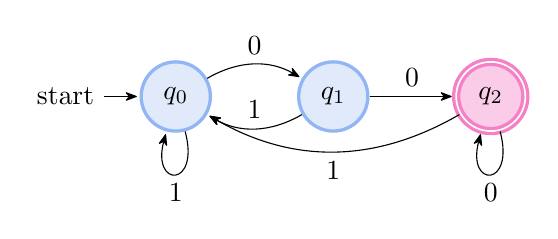
\begin{tikzpicture}[shorten >=1pt,node distance=2cm,on grid,>={Stealth[round]},
        every state/.style={draw=CornflowerBlue!70,fill=CornflowerBlue!20,very thick}, 
        accepting/.style={draw=magenta!50,fill=magenta!20, very thick,double}]
    
      \node[state,initial]  (q_0)                      {$q_0$};
      \node[state]          (q_1) [right=of q_0] {$q_1$};
      \node[state, accepting]          (q_2) [right=of q_1] {$q_2$};
    
      \path[->] (q_0) edge [bend left]             node[above]  {\(0\)} (q_1)
                      edge [loop below]             node  {\(1\)} ()
                (q_1) edge node[above]           {\(0\)} (q_2)
                edge [bend left] node[above] {\(1\)} (q_0) 
                (q_2) edge [loop below] node               {\(0\)} ()
                (q_2) edge [bend left] node[below] {\(1\)} (q_0);
    \end{tikzpicture}
\end{center}We can see that this is quite similar to the previous DFA, except we go back to \(q_0\) when we read a \(1\) in \(q_2\). 
Compare that also to the DFA for a seemingly similar language:\begin{center}
    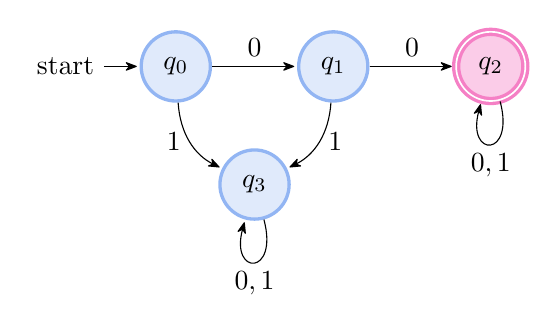
\begin{tikzpicture}[shorten >=1pt,node distance=2cm,on grid,>={Stealth[round]},
        every state/.style={draw=CornflowerBlue!70,fill=CornflowerBlue!20,very thick}, 
        accepting/.style={draw=magenta!50,fill=magenta!20, very thick,double}]
    
      \node[state,initial]  (q_0)                      {\(q_0\)};
      \node[state]          (q_1) [right=of q_0] {\(q_1\)};
      \node[state, accepting]          (q_2) [right=of q_1] {\(q_2\)};
      \node[state] (q_3) at (1, -1.5) {\(q_3\)};
    
      \path[->] (q_0) edge          node[above]  {\(0\)} (q_1)
                      edge [bend right]             node[left]  {\(1\)} (q_3)
                (q_1) edge node[above]           {\(0\)} (q_2)
                edge [bend left] node[right] {\(1\)} (q_3) 
                (q_2) edge [loop below] node               {\(0,1\)} ()
                (q_3) edge [loop below] node               {\(0,1\)} ();
    \end{tikzpicture}
\end{center}
This is a DFA for \(\lang_2 = \{w \in \Sigma^* \mid 00~\text{is a prefix of}~w \}\). 
Obviously, if a string starts with a \(1\), or a \(01\), then it is discarded regardless of what comes after. 
This is represented in the DFA by moving to state \(q_3\) whenever either of these prefixes are read. 
As we can see, once the DFA goes to \(q_3\), there is no way out---this is why such states are often called \emph{trap states}.\endex{}

\exm{} Let's transform the second DFA from the previous example into its table representation. 
We begin at the starting state, \(q_0\). 
From here, given a \(0\), we move to \(q_1\), and given a \(1\) we move to \(q_3\). 
We represent this by a row of information\begin{center}
    \begin{tabular}{c|cc}
        \toprule 
        state & \(0\) & \(1\) \\ 
        \midrule 
        \(\to q_0\) & \(q_1\) & \(q_3\)
    \end{tabular}
\end{center}
Then, in \(q_1\), we move to \(q_2\) given a \(0\) and to \(q_3\) given a \(1\). 
We add this row to our table:
\begin{center}
    \begin{tabular}{c|cc}
        \toprule 
        state & \(0\) & \(1\) \\ 
        \midrule 
        \(\to q_0\) & \(q_1\) & \(q_3\) \\ 
        \(q_1\) & \(q_2 \) & \(q_3\)
    \end{tabular}
\end{center}
We carry on doing this until all states are given rows, leaving us with\begin{center}
    \begin{tabular}{c|cc}
        \toprule 
        state & \(0\) & \(1\) \\ 
        \midrule 
        \(\to q_0\) & \(q_1\) & \(q_3\) \\ 
        \(q_1\) & \(q_2 \) & \(q_3\) \\ 
        \(q_2\to\) & \(q_2\) & \(q_2\) \\ 
        \(q_3\) & \(q_3\) & \(q_3\) \\ 
        \bottomrule
    \end{tabular}
\end{center}
Make sure you convince yourself that this process is reversible. 
Try going from this table back to the DFA.\endex{}

We can now more formally state the reason DFAs are called ``deterministic''. 
Imagine a DFA like this one:\begin{center}
    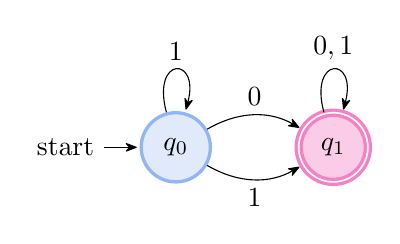
\begin{tikzpicture}[shorten >=1pt,node distance=2cm,on grid,>={Stealth[round]},
        every state/.style={draw=CornflowerBlue!70,fill=CornflowerBlue!20,very thick}, 
        accepting/.style={draw=magenta!50,fill=magenta!20, very thick,double}]
    
      \node[state,initial]  (q_0)                      {\(q_0\)};
      \node[state, accepting]          (q_1) [right=of q_0] {\(q_1\)};
    
      \path[->] (q_0) edge [bend left]          node[above]  {\(0\)} (q_1)
                      edge [bend right]             node[below]  {\(1\)} (q_1)
                      edge [loop above] node {\(1\)} ()
                      (q_1) edge [loop above] node {\(0,1\)} (); 
    \end{tikzpicture}
\end{center}
From state \(q_0\), if we read a \(1\), we can \emph{either} go to \(q_1\) or loop back and stay in \(q_0\). 
Thus, if we take the string \(110\) for example, we have two possible sequences of states we could go through:\[
    q_0 \overset{1}{\to} q_0 \overset{1}{\to} q_1 \overset{0}{\to} q_1 ~\text{or}~q_0 \overset{1}{\to} q_1 \overset{1}{\to} q_1 \overset{0}{\to} q_1. 
\]
There is a choice to be made!
Compare this to all our previous examples, wherein there was exactly one arrow per symbol coming out of each state. 
This property ensures that given an arbitrary input string, there is exactly one way of proceeding through the DFA. 
As it turns out, allowing for multiple transitions per symbol is convenient enough for readability to warrant an entirely new model of computation, that of the \emph{non}deterministic FAs. 
We will take a closer look at these in Section~\ref{sec:nondet}. 

\exm{} All our examples so far have only had one accepting state, but since \(F \subseteq Q\) in general, there may be more than one. 
Take the language \(\lang = \{ w\in\Sigma^* \mid w = 0^m 1^n, m,n\geq 0\}\). 
Recall that in our notation, \(0^m\) means \(m\) \(0\)'s concatenated together. 
The DFA for this language is\begin{center}
    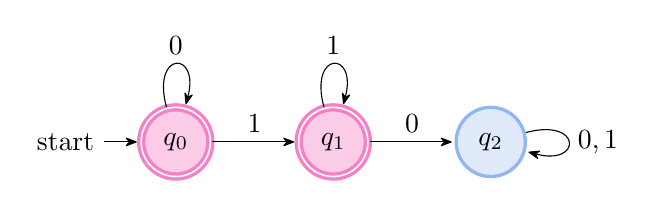
\begin{tikzpicture}[shorten >=1pt,node distance=2cm,on grid,>={Stealth[round]},
        every state/.style={draw=CornflowerBlue!70,fill=CornflowerBlue!20,very thick}, 
        accepting/.style={draw=magenta!50,fill=magenta!20, very thick,double}]
    
      \node[state,initial,accepting]  (q_0)                      {\(q_0\)};
      \node[state, accepting]          (q_1) [right=of q_0] {\(q_1\)};
      \node[state]          (q_2) [right=of q_1] {\(q_2\)};
    
      \path[->] (q_0) edge        node[above]  {\(1\)} (q_1)
                      edge [loop above] node {\(0\)} ()
                      (q_1) edge [loop above] node {\(1\)} ()
                      edge node[above] {\(0\)} (q_2)
                      (q_2) edge [loop right] node {\(0,1\)} (); 
    \end{tikzpicture}
\end{center}In this example, we have \(F = \{q_0, q_1\}\).\endex{}

The next logical step would be to formalize what it means for a DFA to \emph{accept} a string \(w\). 
We will say that a DFA \(\machine\) accepts \(w = a_1 a_2 \cdots a_n\) iff there exists a sequence of states\[q_{(0)} \overset{a_1}{\to} q_{(1)} \overset{a_2}{\to} \cdots \overset{a_n}{\to} q_{(n)}\]so that the first state in the sequence \(q_{(0)} = q_0\) is initial and the last state \(q_{(n)} \in F\) is accepting, and for each \(a_i\),\[
    \delta(q_{(i-1)}, a_i) = q_{(i)}. 
\]This definition looks intimidating, but all it is saying is that each state in the sequence of states follows the previous one based on the transition function. 

\exm{} Let's look back at our very first example.\begin{center}
    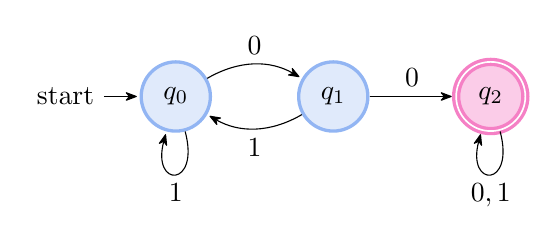
\begin{tikzpicture}[shorten >=1pt,node distance=2cm,on grid,>={Stealth[round]},
        every state/.style={draw=CornflowerBlue!70,fill=CornflowerBlue!20,very thick}, 
        accepting/.style={draw=magenta!50,fill=magenta!20, very thick,double}]
    
      \node[state,initial]  (q_0)                      {$q_0$};
      \node[state]          (q_1) [right=of q_0] {$q_1$};
      \node[state, accepting]          (q_2) [right=of q_1] {$q_2$};
    
      \path[->] (q_0) edge [bend left]             node[above]  {\(0\)} (q_1)
                      edge [loop below]             node  {\(1\)} ()
                (q_1) edge node[above]           {\(0\)} (q_2)
                edge [bend left] node[below] {\(1\)} (q_0) 
                (q_2) edge [loop below] node               {\(0,1\)} ();
    \end{tikzpicture}
\end{center}
Earlier, we went through a step-by-step procedure of accepting the string \(1001\). 
We moved in the sequence\[
q_0 \overset{1}{\to} q_0 \overset{0}{\to} q_1 \overset{0}{\to}  q_2 \overset{1}{\to} q_2.
\]In this case, we do have that the first state in the sequence \(q_{(0)} = q_0\) is initial, and the last state in the sequence \(q_{(5)} = q_2 \in F\) is final. 
We also know from our diagram that at each state in this sequence, the transition (indicated here by the symbol above each arrow) is valid, i.e., that \(\delta(q_{(i-1)}, a_i) = q_{(i)}\). 
For instance, note that \(a_2 = 0\) and \(q_{(1)} = q_0\), and we know that \(\delta(q_0, 0) = q_1\), which is precisely \(q_{(2)}\) in the sequence.\endex{} 

\vspace{10pt}
\begin{minipage}{.14\textwidth}
    \includegraphics[width=2cm]{nerd_maddy.png} 
\end{minipage}%
\fcolorbox{Periwinkle}{white!100}{
\begin{minipage}{.76\textwidth}
    \textbf{Nerd Interjection!} The distinction between \(q_{(i)}\) for the \(i^\text{th}\) state in a \emph{sequence} of states and \(q_i\) for the \(i^\text{th}\) state in a \emph{DFA} is quite unfortunate notation for legibility, but its faily standard. 
    In any case, there's not really any rule dictating that we need to use \(q_i\) for states, so feel free to use \(a, b, c, \ldots\) instead. 
    Just make sure the symbols you use aren't part of the alphabet, otherwise it can get \textit{really} confusing! 
\end{minipage}}
\vspace{10pt}

All of that is just a math-y way of saying what us computer scientists understand fairly well as a condition known as ``this algorithm terminates with this outcome''. 
So, if you'd like, you can instead view the outcome of a DFA processing a string as the outcome of this algorithm:\begin{center}\begin{minipage}{0.6\textwidth}
    \begin{algorithm}[H]
        \label{alg:1.1.1}
        % \SetArgSty{}
        \caption{The process of accepting or rejecting a string}
        \KwIn{a string \(w = a_1 a_2 \cdots a_n\) and a DFA \(\machine\)}
        \KwOut{either \textsc{accept} or \textsc{reject}} 
        \(q_\text{curr} \gets q_0\)\; 
        \For{\(a_i\) \textbf{in} \(w\)}{
            \(q_\text{curr} \gets \delta (q_\text{curr}, a_i)\)\; 
        }
        \If{\(q_\text{curr} \in F\)}{
            \Return{\textsc{accept}}\;
        }\Return{\textsc{reject}}\;
    \end{algorithm}
\end{minipage}
\end{center}

Indeed, this algorithm terminating with \textsc{accept} is equivalent to the definition we gave earlier of there being an accepting sequence of states, so we can generally adopt either of them as our definition for ``DFA \(\machine\) accepts the string \(w\)''. 
We can even give a \emph{third} formulation using recursion. 
We construct a new function \(\hat\delta: Q \times \Sigma^* \to Q\), which, instead of operating over single symbols, takes in as input entire strings. The function is defined as follows:\begin{enumerate}
    \item if \(w = a\) for some \(a\in \Sigma\), then \(\hat\delta (q_i, a) = \delta (q_i, a)\); and 
    \item if \(w = a_1 a_2 \cdots a_k\) for some \(a_i \in \Sigma\), then \(\hat\delta(q_i, w) = \delta\big(\hat\delta (q_i, a_1 a_2 \cdots a_{k-1}), a_k\big)\). 
\end{enumerate}
Intuitively, all \(\hat\delta\) does is recursively backtrack until it hits the first symbol, and then iterates through every symbol after that---just like Algorithm~\ref{alg:1.1.1}. 
Then, we can say that a DFA accepts a string \(w\) iff \(\hat\delta (q_0, w) \in F\) is an accepting state. 
This definition too is equivalent to our previous ones, and its generally the one we will adopt, if only for notational convenience. 

Now that we've clarified what it means for a DFA to accept a string, we can define \(\lang(\machine)\) to be the set of all strings accepted by a certain DFA \(\machine\), also known as its language. 
We will say that \(\machine\) \emph{recognizes} \(\lang\) whenever \(\lang = \lang(\machine)\).
We've mostly been providing languages and trying to find DFAs for them, but let's see how we might go the other way around. 

\exm{} Let \(\machine\) be the following DFA:\begin{center}
    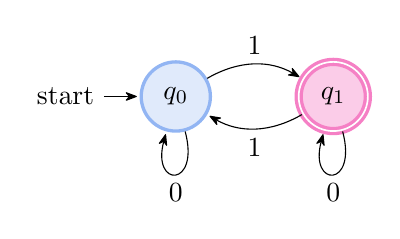
\begin{tikzpicture}[shorten >=1pt,node distance=2cm,on grid,>={Stealth[round]},
        every state/.style={draw=CornflowerBlue!70,fill=CornflowerBlue!20,very thick}, 
        accepting/.style={draw=magenta!50,fill=magenta!20, very thick,double}]
    
      \node[state,initial]  (q_0)                      {$q_0$};
      \node[state,accepting]          (q_1) [right=of q_0] {$q_1$};
    
      \path[->] (q_0) edge [bend left]             node[above]  {\(1\)} (q_1)
                      edge [loop below]             node  {\(0\)} ()
                (q_1) edge[bend left] node[below]           {\(1\)} (q_0)
                edge [loop below] node {\(0\)} ();
    \end{tikzpicture}
\end{center}
Let's try and figure out what language this DFA recognizes. 
We can see that reading a \(0\) makes the computation stay in place, so we can safely assume that the language does not distinguish anything about \(0\)'s, but it switches from accept to non-accept every time it reads a \(1\). 
It rejects \(\varepsilon\), accepts \(1\), rejects \(11\), accepts \(111\), rejects \(1111\), and so on---it seems to be alternating depending on how many \(1\)'s there are in the string. 
Thus, \(\lang(\machine) = \{w \in \Sigma^*\mid w~\text{has an odd number of}~1\text{'s}\}\).\endex{}

You might be wondering if there's a way to classify what sorts of languages can be recognized by a DFA without directly referring to a DFA. 
We'll look at this question more in depth in Section~\ref{sec:regex}, but for now let's have the following definition: call a language over an alphabet \(\Sigma\) \emph{regular} iff there exists some DFA that recognizes that language. 

\exm{} Here's another language that a DFA can recognize. 
Let \(\Sigma = \{0, 1, 2, 3, 4, 5, 6, 7, 8, 9\}\) be the set of digits in base 10. 
Thus, strings in \(\Sigma^*\) are just decimal numbers (with some weirdo ones like \(000\) or \(001\), but we can just ignore leading \(0\)'s). 
We'll show that the language \(\lang = \{w \in \Sigma^* \mid w~\text{is divisible by}~3\}\) is a regular language, by giving this DFA:\begin{center}
    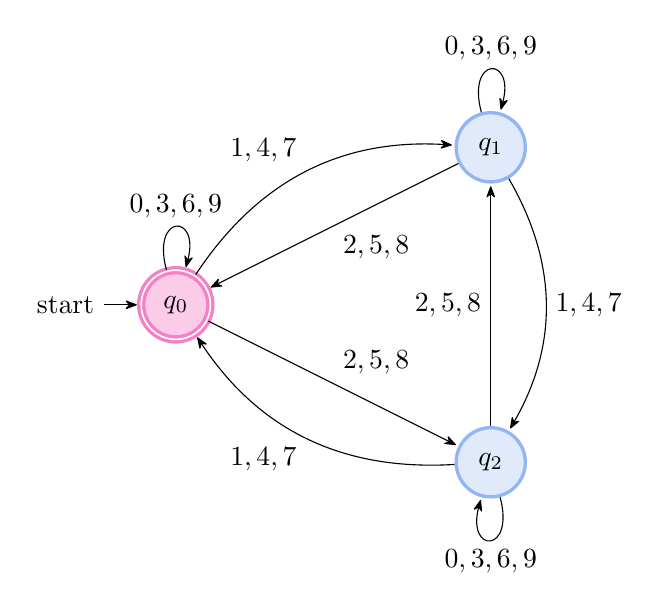
\begin{tikzpicture}[shorten >=1pt,node distance=3cm,on grid,>={Stealth[round]},
        every state/.style={draw=CornflowerBlue!70,fill=CornflowerBlue!20,very thick}, 
        accepting/.style={draw=magenta!50,fill=magenta!20, very thick,double}]
    
      \node[state,initial,accepting]  (q_0)                      {\(q_0\)};
      \node[state]        (q_1) at (4,2) {\(q_1\)};
      \node[state]          (q_2) at (4,-2) {\(q_2\)};
    
      \path[->] (q_0) edge [bend left]        node[above left]  {\(1,4,7\)} (q_1)
                      edge [loop above] node {\(0,3,6,9\)} ()
                      edge  node[above right] {\(2,5,8\)} (q_2)
                      (q_1) edge [loop above] node {\(0,3,6,9\)} ()
                      edge[bend left] node[right] {\(1,4,7\)} (q_2)
                      edge node[below right] {\(2,5,8\)} (q_0)
                      (q_2) edge [loop below] node {\(0,3,6,9\)} ()
                      edge node[left] {\(2,5,8\)} (q_1)
                      edge[bend left] node[below left] {\(1,4,7\)} (q_0); 
    \end{tikzpicture}
\end{center}
Recall that to tell if a number is divisible by \(3\), we simply add up the digits and check if \textit{that} is divisble by \(3\). 
What this machine is doing is keeping track of the remainder \(\bmod ~3\) of the ``running total'' of the digits!
Say our number is \(3147\). 
The DFA reads a \(3\), so the running total is \(3\), which is divisible by \(3\), so we stay in state \(q_0\). 
Next, we read a \(1\), which makes our running total \(4\). 
\(4\bmod 3\) is \(1\), so we go to state \(q_1\). 
Next, we read a \(4\), which makes our running total \(8\).
\(8\bmod 3\) is \(2\), so we go to state \(q_2\). 
Finally, we read a \(7\), putting our final sum of digits at \(15\)---which is divisible by \(3\)!
This is reflected in the fact that the DFA sends us to state \(q_0\) again, the only accepting state, so we accept \(3147\).\endex{}

Via the correspondence we established in Chapter~\ref{ch:intro} between decision problems and languages, we can say that DFAs can solve the problem of deciding whether or not a number in base \(10\) is divisible by \(3\). 
Quite impressive! 
With just a few states and a few instructions, we can tell this machine to completely solve this problem.
Of course, this is quite an easy problem. 
How about a problem that a DFA \textit{can't} solve? 

\section{Closure properties}
Languages, being sets, can be operated on using established set operations. 

\exm{} Consider the languages \(\lang_1 = \{w \in \Sigma^* \mid 00~\text{is a suffix of}~w\} \) and \(\lang_2 = \{w\in\Sigma^* \mid w~\text{starts with}~1 \}\). 
These are both regular. 
Their intersection \(\lang_1 \cap \lang_2\) would be the set of all strings who start with \(1\) and end in \(00\). 
The first few elements can be listed:\[
\lang_1 \cap \lang_2 = \{ 100, 1000, 1100, 10000, 10100, 11000, 111000, \ldots \}. 
\] \endex{}

A natural question arises: is the result of applying an operation to one or two regular languages still a regular language? 
Mathematically, when a type of object satisfies this property, we say that the objects are \emph{closed} under the operation. 
The prototypical example is the natural numbers, which are closed under addition (\(2 + 3 = 5\) and so on) but not closed under subtraction (\(2 - 3 = -1\), not a natural number). 

The answer, as we will see later, is yes, in the cases of regular set operations. 
Before we prove these statements in the general case, though, let's think of what we would do given a particular DFA for the case of a set complement. 
Recall that \(\lang^\complement\) is the set of all strings over the same alphabet \(\Sigma\) as \(\lang\) but are not themselves members of \(\lang\). 
Since we established that a language is regular whenever a DFA recognizes it, if we want to show that \(\lang^\complement\) is also regular, we need to construct a DFA for it, and we need to do so only given the data of the DFA for \(\lang\). 
This turns out to be fairly straightforward. 

\exm{} Consider the DFA \(\machine\):\begin{center}
    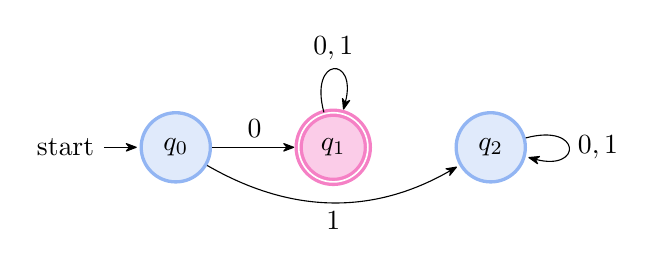
\begin{tikzpicture}[shorten >=1pt,node distance=2cm,on grid,>={Stealth[round]},
        every state/.style={draw=CornflowerBlue!70,fill=CornflowerBlue!20,very thick}, 
        accepting/.style={draw=magenta!50,fill=magenta!20, very thick,double}]
    
      \node[state,initial]  (q_0)                      {\(q_0\)};
      \node[state,accepting]          (q_1) [right=of q_0] {\(q_1\)};
      \node[state]       (q_2) [right=of q_1] {\(q_2\)};
    
      \path[->] (q_0) edge          node[above]  {\(0\)} (q_1)
                      edge [bend right]             node[below]  {\(1\)} (q_2)
                (q_1) edge [loop above] node           {\(0,1\)} ()
                (q_2) edge [loop right] node               {\(0,1\)} ();
    \end{tikzpicture}
\end{center}
Note that \(\lang(\machine)\) is all strings that start with \(0\). 
If we want to accept those strings that \(\machine\) rejects, then we can simply modify \(\machine\) to accept on every non-accepting state, and reject on every accepting state. 
This process yields the new DFA \(\machine'\):\begin{center}
    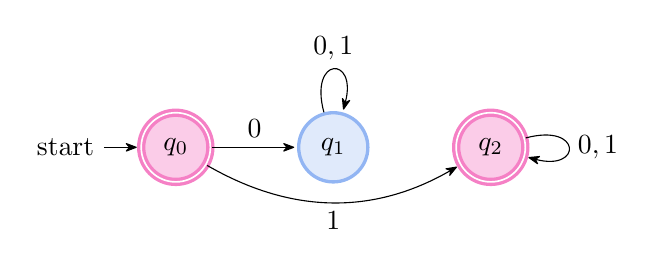
\begin{tikzpicture}[shorten >=1pt,node distance=2cm,on grid,>={Stealth[round]},
        every state/.style={draw=CornflowerBlue!70,fill=CornflowerBlue!20,very thick}, 
        accepting/.style={draw=magenta!50,fill=magenta!20, very thick,double}]
    
      \node[state,initial,accepting]  (q_0)                      {\(q_0\)};
      \node[state]          (q_1) [right=of q_0] {\(q_1\)};
      \node[state,accepting]       (q_2) [right=of q_1] {\(q_2\)};
    
      \path[->] (q_0) edge          node[above]  {\(0\)} (q_1)
                      edge [bend right]             node[below]  {\(1\)} (q_2)
                (q_1) edge [loop above] node           {\(0,1\)} ()
                (q_2) edge [loop right] node               {\(0,1\)} ();
    \end{tikzpicture}
\end{center}
It is then clear that \(\lang(\machine')\) is all strings that start with \(1\), plus the empty string, which is precisely \({\lang(\machine)}^\complement\).\endex{}

Let's reflect on what we just did. 
In order to obtain a machine for the complement of a language given a machine for that language, we simply retained all of the original states, the alphabet, the initial state, and the transition function, then flipped all accepting states into non-accepting states and vice-versa. 
It's not hard to see that this argument works out no matter what the ``underlying'' DFA is: if in the original DFA \(\machine\), computation terminates in an accepting state, then in the new \(\machine'\), computation would terminate in a non-accepting state. 
We formalize this with the following theorem. 

\begin{theorem}[Closure under complements]
    The complement \(\lang^\complement \) of a regular language \(\lang\) is itself a regular language. 
\end{theorem}

\begin{proof}
    Let \(\lang\) be a regular language, and \(\machine = \langle Q, \Sigma, \delta, q_0 , F\rangle\) be its corresponding DFA. 
    Then, we can construct a new DFA \(\machine'\) for \(\lang^\complement\) by taking\[
    \machine' = \langle Q, \Sigma, \delta, q_0, Q - F \rangle
    \]where \(Q - F\) is the set of all non-accepting states in \(\machine\). 
    Then, \(\lang^\complement = \lang(\machine')\), for if the result of \(\hat\delta(q_0, w) = q_n\in F\) is an accepting state in \(\machine\), then this state \(q_n\) will not be in \(Q -F\), so \(\machine'\) will not accept \(w\).
\end{proof}

\section{Nondeterminism}\label{sec:nondet}

As we can see at the end of the last section, it's going to be quite difficult to prove that the regular languages are closed under string operations just by using DFAs. 
If we could allow for transitions \textit{without} reading any character, then both these problems are very easily solved: given languages \(\lang_1\) and \(\lang_2\), and corresponding DFAs \(\machine_1\) and \(\machine_2\), we can construct a machine for \(\lang_1 \lang_2\) by adding these \(\varepsilon\)-transitions from every final state of \(\machine_1\) to the starting state of \(\machine_2\). 

This introduces new problems, however: now, there is no unique way of computing a certain string. 
It's easy to see why, as in the following example.

\exm{} Consider the two languages \(\lang_1 = \{ w \in \Sigma^* \mid w~\text{contains at least two}~0\text{'s} \}\) and \(\lang_2 = \{ w \in \Sigma^* \mid w~\text{starts and ends with the same symbol} \} \). 
Construct a new machine using \(\machine_1\) and \(\machine_2\) using the process outlined above, giving us something like:\begin{center}
    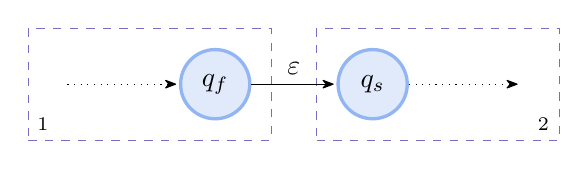
\begin{tikzpicture}[shorten >=1pt,node distance=2cm,on grid,>={Stealth[round]},
        every state/.style={draw=CornflowerBlue!70,fill=CornflowerBlue!20,very thick}, 
        accepting/.style={draw=magenta!50,fill=magenta!20, very thick,double}]
    
      \node[state]  (q_f1)                      {\(q_{f}\)};
      \node[state]          (q_i2) [right=of q_f1] {\(q_{s}\)};
      \node (m2) [right=of q_i2] {}; 
      \node (m1) [left=of q_f1] {}; 
      \node[draw=Periwinkle,dashed,fit=(q_f1) (m1), inner sep=0.25cm] (machine1) {}; 
      \node[draw=Periwinkle,dashed,fit=(q_i2) (m2), inner sep=0.25cm] (machine2) {}; 
      \node[above right] at (machine1.south west) {\(\machine_1\)};
      \node[above left] at (machine2.south east) {\(\machine_2\)};
    
      \path[->] (q_f1) edge          node[above]  {\(\varepsilon\)} (q_i2);
      \path[dotted,->] (m1) edge (q_f1);
      \path[dotted,->] (q_i2) edge (m2); 
    \end{tikzpicture}
\end{center}
Then, given a string like \(00100\), we can parse it in \textit{at least} two different ways: either as \(001\) concatenated with \(00\)---which is a member of \(\lang_1 \lang_2\)---or as \(00\) concatenated with \(100\)---which isn't a member of \(\lang_1 \lang_2\). 
We will be at the final state of \(\machine_1\) by the time we finish reading \(00\), and we can choose to transition to \(\machine_2\) either after reading a \(1\) or before reading the \(1\). Visually,\begin{center}
    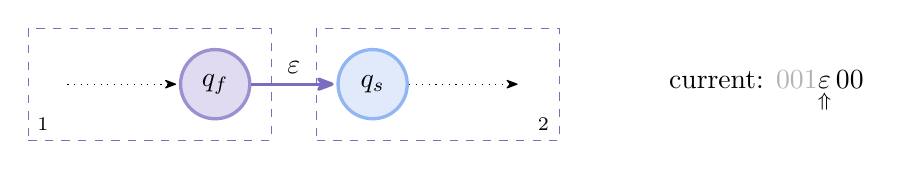
\begin{tikzpicture}[shorten >=1pt,node distance=2cm,on grid,>={Stealth[round]},
        every state/.style={draw=CornflowerBlue!70,fill=CornflowerBlue!20,very thick}, 
        accepting/.style={draw=purple!50,fill=purple!20, very thick,double}]
    
      \node[state,draw=Periwinkle!70,fill=Periwinkle!20]  (q_f1)                      {\(q_{f}\)};
      \node[state]          (q_i2) [right=of q_f1] {\(q_{s}\)};
      \node (m2) [right=of q_i2] {}; 
      \node (m1) [left=of q_f1] {}; 
      \node[draw=Periwinkle,dashed,fit=(q_f1) (m1), inner sep=0.25cm] (machine1) {}; 
      \node[draw=Periwinkle,dashed,fit=(q_i2) (m2), inner sep=0.25cm] (machine2) {}; 
      \node[above right] at (machine1.south west) {\(\machine_1\)};
      \node[above left] at (machine2.south east) {\(\machine_2\)};
      \node (word) at (7,-0.1)  {current: \(\textcolor{black!30}{001}\underset{\Uparrow}{\varepsilon}\,00\)};
    
      \path[->] (q_f1) edge[very thick, draw=Periwinkle]          node[above]  {\(\varepsilon\)} (q_i2);
      \path[dotted,->] (m1) edge (q_f1);
      \path[dotted,->] (q_i2) edge (m2); 
    \end{tikzpicture}

    versus

    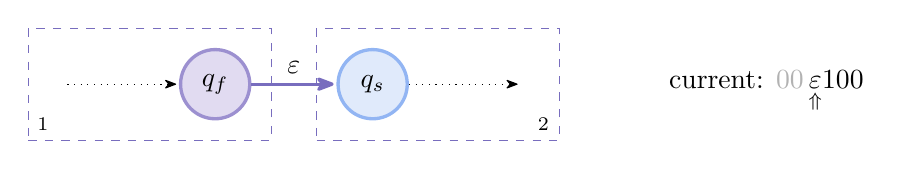
\begin{tikzpicture}[shorten >=1pt,node distance=2cm,on grid,>={Stealth[round]},
        every state/.style={draw=CornflowerBlue!70,fill=CornflowerBlue!20,very thick}, 
        accepting/.style={draw=purple!50,fill=purple!20, very thick,double}]
    
      \node[state,draw=Periwinkle!70,fill=Periwinkle!20]  (q_f1)                      {\(q_{f}\)};
      \node[state]          (q_i2) [right=of q_f1] {\(q_{s}\)};
      \node (m2) [right=of q_i2] {}; 
      \node (m1) [left=of q_f1] {}; 
      \node[draw=Periwinkle,dashed,fit=(q_f1) (m1), inner sep=0.25cm] (machine1) {}; 
      \node[draw=Periwinkle,dashed,fit=(q_i2) (m2), inner sep=0.25cm] (machine2) {}; 
      \node[above right] at (machine1.south west) {\(\machine_1\)};
      \node[above left] at (machine2.south east) {\(\machine_2\)};
      \node (word) at (7,-0.1)  {current: \(\textcolor{black!30}{00}\,\underset{\Uparrow}{\varepsilon}100\)};
    
      \path[->] (q_f1) edge[very thick, draw=Periwinkle]          node[above]  {\(\varepsilon\)} (q_i2);
      \path[dotted,->] (m1) edge (q_f1);
      \path[dotted,->] (q_i2) edge (m2); 
    \end{tikzpicture}
\end{center}
This is because \(\machine_1\) will accept both \(00\) and \(001\)---and, in fact, \(0010\) and \(00100\) as well! 
We can't know for sure when we should take the epsilon transition to lead to an accepting computation, but we know that it \textit{should} be accepted. 
The choice here is important, as it makes all the difference between an accepting computation and a non-accepting one!\endex{} 

This means that the introduction of \(\varepsilon\)-transitions causes our machines to be \textit{nondeterministic}, which calls for a general defintion of a \emph{nondeterministic finite automaton}, or an \emph{NFA}. 

\vspace{10pt}
\begin{minipage}{.14\textwidth}
    \includegraphics[width=2cm]{nerd_maddy.png} 
\end{minipage}%
\fcolorbox{Periwinkle}{white!100}{
\begin{minipage}{.76\textwidth}
    \textbf{Nerd Interjection!} As it turns out, NFAs without \(\varepsilon\)-transitions are significantly different enough from those \textit{with} \(\varepsilon\)-transitions that we will treat them as separate kinds of machines, distinguishing between general NFAs and \(\varepsilon\)-NFAs respectively. 
    The introduction of \(\varepsilon\)-transitions complicates the conversion process from NFAs to DFAs (spoilers!) that we will look at later. 
\end{minipage}}
\vspace{10pt}

An NFA \(\machine\) consists of the following data:\begin{enumerate}
    \item a finite set of states \(Q\); 
    \item an alphabet of allowed symbols \(\Sigma\); 
    \item a transition function \(\delta : Q \times \Sigma \to \mathcal{P}(Q)\) to the \emph{powerset} of \(Q\); 
    \item an initial state \(q_0\); and 
    \item a subset \(F\subseteq Q\) of final states. 
\end{enumerate}
The main difference (in fact, the only difference) between the description of a DFA to an NFA is the transition function: instead of only returning one state for every state-symbol pair, we return a \textit{set} of states. 
This, in particular, means that we can also return nothing---given a state and a symbol, there may be no other way to move to a different state. 
This written as \(\delta(q, a) = \{\}\), the empty set. 
If we want to transform the definition into one for an \(\varepsilon\)-NFA, then we simply add \(\varepsilon\) to the alphabet \(\Sigma\). 

Convince yourself that the transition function taking values in the powerset of \(Q\) instead of elements of \(Q\) precisely captures the notion of nondeterminism. 
For, say that given a state-symbol pair, \(\delta (q, a) = \{q_1, q_3, q_4 \}\). 
Which one of the three states in the set would we transition to next? 
There is a choice to be made here, which complicates our computation---but greatly simplifies the presentation of NFAs. 

\exm{} Consider the language \(\lang = \{ 1 0^m 1 \mid m \ge 0 \}\). 
This is an NFA for this language:\begin{center}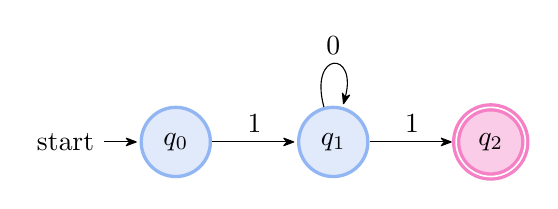
\begin{tikzpicture}[shorten >=1pt,node distance=2cm,on grid,>={Stealth[round]},
    every state/.style={draw=CornflowerBlue!70,fill=CornflowerBlue!20,very thick}, 
    accepting/.style={draw=magenta!50,fill=magenta!20, very thick,double}]

    \node[state, initial] (q_0) {\(q_0\)}; 
    \node[state] (q_1) [right=of q_0] {\(q_1\)}; 
    \node[state, accepting] (q_2) [right=of q_1] {\(q_2\)}; 

    \path[->] (q_0) edge node[above] {\(1\)} (q_1)
                    (q_1) edge[loop above] node[above] {\(0\)} ()
                    edge node[above] {\(1\)} (q_2); 
\end{tikzpicture}
\end{center}This NFA shows clearly what language its computing---a \(1\), followed by any number of \(0\)'s, and ended with a \(1\). 
If it were a DFA, think of how many more transitions we'd have, as well as at least one more state for trapping the unwanted strings.

In general, if we terminate computation of a string in an NFA with nowhere else to go, but with symbols still left to be read, we consider that a reject. 
So, for instance, \(1011\) will be rejected by this NFA because the computation will terminate in \(q_2\) with a \(1\) leftover.\endex%

We've established that because of nondeterminism, we lose the uniqueness of a computation sequence given a certain string; since transitions can go to multiple states, there likewise might exist multiple ways of processing the same string. 
Visually, we can imagine that while computation in a DFA is a straight line:
\begin{center}
    \tikz[>={Stealth[round]}]\graph[math nodes]{
        q_0 -> q_1 ->[dashed] q_i ->[dashed] q_n
      };
\end{center}computation in an NFA is a \textit{tree}, with many branching paths:
\begin{center}
    \tikz[>={Stealth[round]}]\graph[math nodes]{
        q_0 -> {
            q_1 ->[dashed] q_i, 
            q_2 ->[dashed] {q_j, q_k ->[dashed] q_n} }
      };
\end{center}
This is due to the fact that there can be multiple transitions from each state per character, and not all of these may lead to an accepting computation. 
If any \textit{one} of these paths terminates in an accepting state, and with the whole string consumed, then we will say that the NFA accepts that string. 
This intuitive notion is enough to grasp the formal definition of what it means for an NFA to accept a certain string (like the one we set out for DFAs), so we won't go over it in too much detail here. 

\exm{} Consider the language \(\lang = \{w \in \Sigma^* \mid 01~\text{is a suffix of}~w\}\). An NFA for this is:\begin{center}
    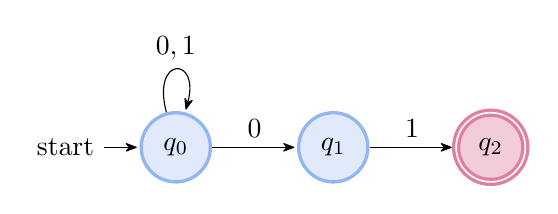
\begin{tikzpicture}[shorten >=1pt,node distance=2cm,on grid,>={Stealth[round]},
        every state/.style={draw=CornflowerBlue!70,fill=CornflowerBlue!20,very thick}, 
        accepting/.style={draw=purple!50,fill=purple!20, very thick,double}]
        
        \node[state, initial] (q_0) {\(q_0\)}; 
        \node[state] (q_1) [right=of q_0] {\(q_1\)}; 
        \node[state, accepting] [right=of q_1] (q_2) {\(q_2\)}; 

        \path[->] (q_0) edge[loop above] node[above] {\(0,1\)} ()
                    edge node[above] {\(0\)} (q_1) 
                    (q_1) edge node[above] {\(1\)} (q_2); 
    \end{tikzpicture}
\end{center}Consider the string \(0101\). 
Verify that there are three possible sequences of states that this machine can go through for this word:\[
    q_0 \to q_0 \to q_0 \to q_0,~~q_0 \to q_0 \to q_1 \to q_2,~\text{and}~~q_1 \to q_2.
\]Of these, only the second sequence both (1) terminates in a final state, and (2) consumes all the symbols in the string. 
However, as we said, so long as \textit{one} of these sequences terminates, the NFA will accept the string. 

Now consider the string \(100\). 
We again have three possible sequences of states:\[
    q_0 \to q_0 \to q_0, ~~q_0 \to q_0 \to q_1,~\text{and}~~q_0 \to q_1.
\]Here, none of these fulfill our criteria for acceptance, so this string will be rejected by the NFA, as desired.\endex%

The usefulness of NFAs in proving things about regular languages lies in the following theorem: 

\begin{theorem}[Equivalence of NFAs and DFAs]\label{theo:equiv-nfa-dfa}
    A language \(\lang \subseteq \Sigma^*\) recognized by an NFA \(\machine\) is a regular language, i.e., there exists a DFA \(\machine'\) that also recognizes \(\lang\), and does so with \(O(2^{|Q|})\) states, where \(Q\) is the set of states of \(\machine\). 
\end{theorem}

Before we prove this, let's look at an example. 
The main idea behind constructing a DFA \(\machine'\) for an NFA \(\machine\) will be to make a state for each possible \textit{subset} of the states of the NFA.
For instance, if there are states \(q_0\) and \(q_1\) in the NFA, there will be states \(\{q_0\}\), \(\{q_1\}\), and \(\{q_0, q_1\}\) in the DFA (and also one for \(\{\}\)). 
Then, to form the transition function, we take the \textit{union} of the outcomes of the NFA's transition function (remember, it returns a set!) for each of the NFA states inside the DFA's states. 

\exm{} Consider the following NFA:\begin{center}
    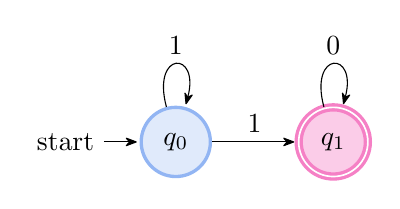
\begin{tikzpicture}[shorten >=1pt,node distance=2cm,on grid,>={Stealth[round]},
        every state/.style={draw=CornflowerBlue!70,fill=CornflowerBlue!20,very thick}, 
        accepting/.style={draw=magenta!50,fill=magenta!20, very thick,double}]
        
        \node[state,initial] (q_0) {\(q_0\)}; 
        \node[state,accepting] (q_1) [right=of q_0] {\(q_1\)}; 

        \path[->] (q_0) edge [loop above] node {\(1\)} ()
                edge node[above] {\(1\)} (q_1) 
                (q_1) edge [loop above] node {\(0\)} (); 
    \end{tikzpicture}
\end{center} Let this NFA be \(\machine = \langle Q, \Sigma, \delta, q_0, F \rangle\). 
We construct the states of the DFA \(\machine'\) piece by piece (except the transition function, which we save for last):\begin{enumerate}
    \item the states of \(\machine'\) will be \(\mathcal{P(Q)}\); 
    \item the alphabet \(\Sigma\) will remain the same; 
    \item the starting state will be the set containing \(q_0\), so \(\{q_0\}\); 
    \item the final states will be any subset of \(Q\) which contains a state from \(F\), so in this case, \(\{q_0, q_1\}\) and \(\{q_1\}\). 
\end{enumerate} This gives us the following picture: 
\begin{center}
    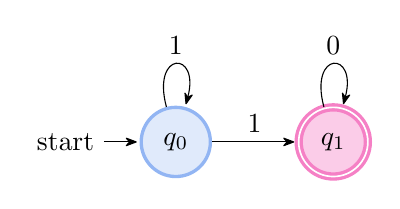
\begin{tikzpicture}[shorten >=1pt,node distance=2cm,on grid,>={Stealth[round]},
        every state/.style={draw=CornflowerBlue!70,fill=CornflowerBlue!20,very thick}, 
        accepting/.style={draw=magenta!50,fill=magenta!20, very thick,double},
        baseline=(current bounding box.center)]
        
        \node[state,initial] (q_0) {\(q_0\)}; 
        \node[state,accepting] (q_1) [right=of q_0] {\(q_1\)}; 

        \path[->] (q_0) edge [loop above] node {\(1\)} ()
                edge node[above] {\(1\)} (q_1) 
                (q_1) edge [loop above] node {\(0\)} (); 
    \end{tikzpicture}
    \hspace{20pt}
    \begin{tikzpicture}[shorten >=1pt,node distance=2cm,on grid,>={Stealth[round]},baseline=(current bounding box.center)]
        \path[dashed,->] (0,0) edge (1.5,0); 
    \end{tikzpicture}
    \hspace{20pt}
    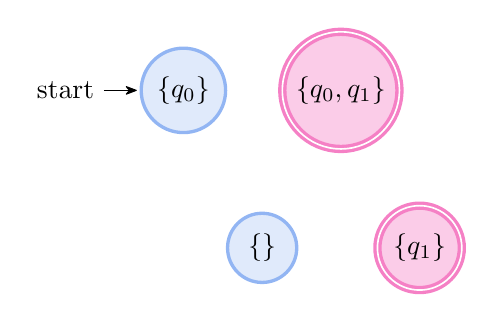
\begin{tikzpicture}[shorten >=1pt,node distance=2cm,on grid,>={Stealth[round]},
        every state/.style={draw=CornflowerBlue!70,fill=CornflowerBlue!20,very thick}, 
        accepting/.style={draw=magenta!50,fill=magenta!20, very thick,double},
        baseline=(current bounding box.center)]
        
        \node[state,initial] (q_0) {\(\{q_0\}\)}; 
        \node[state,accepting] (q_01) [right=of q_0] {\(\{q_0, q_1\}\)};
        \node[state] (emp) at (1, -2) {\(\{\}\)}; 
        \node[state,accepting] (q_1) [right=of emp] {\(\{q_1\}\)};
    \end{tikzpicture}
\end{center} I'll keep the old NFA off to the side so we can consult it while we construct our new machine. 

Now we go about filling in the arrows between the states. 
To do this, we simply start at \(\{q_0\}\) and make transitions ``as needed''. 
Remember, our general strategy will be to take the union of all the possible outputs under \(\delta\) for each NFA state within the DFA states. 
So for \(\{q_0\}\), its only member is, well, \(q_0\). 
In the NFA, reading a \(1\) at \(q_0\) leads us either to \(q_0\) or \(q_1\), so we represent this by drawing the following arrow in our DFA:\begin{center}
    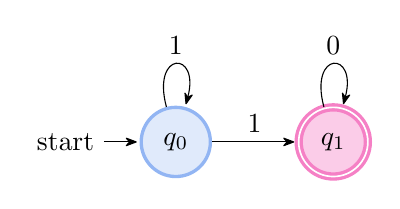
\begin{tikzpicture}[shorten >=1pt,node distance=2cm,on grid,>={Stealth[round]},
        every state/.style={draw=CornflowerBlue!70,fill=CornflowerBlue!20,very thick}, 
        accepting/.style={draw=magenta!50,fill=magenta!20, very thick,double},
        baseline=(current bounding box.center)]
        
        \node[state,initial] (q_0) {\(q_0\)}; 
        \node[state,accepting] (q_1) [right=of q_0] {\(q_1\)}; 

        \path[->] (q_0) edge [loop above] node {\(1\)} ()
                edge node[above] {\(1\)} (q_1) 
                (q_1) edge [loop above] node {\(0\)} (); 
    \end{tikzpicture}
    \hspace{20pt}
    \begin{tikzpicture}[shorten >=1pt,node distance=2cm,on grid,>={Stealth[round]},baseline=(current bounding box.center)]
        \path[dashed,->] (0,0) edge (1.5,0); 
    \end{tikzpicture}
    \hspace{20pt}
    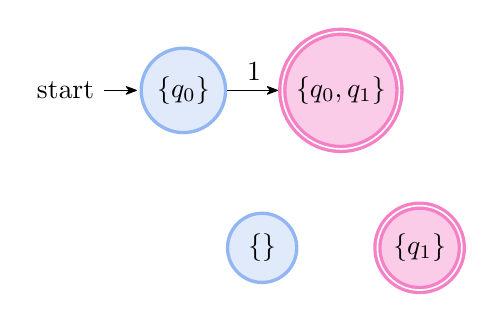
\begin{tikzpicture}[shorten >=1pt,node distance=2cm,on grid,>={Stealth[round]},
        every state/.style={draw=CornflowerBlue!70,fill=CornflowerBlue!20,very thick}, 
        accepting/.style={draw=magenta!50,fill=magenta!20, very thick,double},baseline=(current bounding box.center)]
        
        \node[state,initial] (q_0) {\(\{q_0\}\)}; 
        \node[state,accepting] (q_01) [right=of q_0] {\(\{q_0, q_1\}\)};
        \node[state] (emp) at (1, -2) {\(\{\}\)}; 
        \node[state,accepting] (q_1) [right=of emp] {\(\{q_1\}\)};

        \path[->] (q_0) edge node[above] {\(1\)} (q_01); 
    \end{tikzpicture}
\end{center}Reading a \(0\) while at \(q_0\), on the other hand, doesn't have a corresponding transition! 
We represent this by drawing a transition to the empty set state. 
\begin{center}
    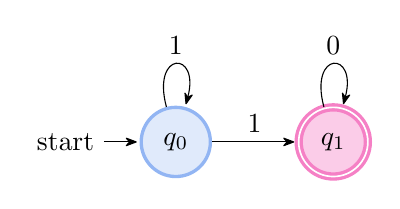
\begin{tikzpicture}[shorten >=1pt,node distance=2cm,on grid,>={Stealth[round]},
        every state/.style={draw=CornflowerBlue!70,fill=CornflowerBlue!20,very thick}, 
        accepting/.style={draw=magenta!50,fill=magenta!20, very thick,double},
        baseline=(current bounding box.center)]
        
        \node[state,initial] (q_0) {\(q_0\)}; 
        \node[state,accepting] (q_1) [right=of q_0] {\(q_1\)}; 

        \path[->] (q_0) edge [loop above] node {\(1\)} ()
                edge node[above] {\(1\)} (q_1) 
                (q_1) edge [loop above] node {\(0\)} (); 
    \end{tikzpicture}
    \hspace{20pt}
    \begin{tikzpicture}[shorten >=1pt,node distance=2cm,on grid,>={Stealth[round]},baseline=(current bounding box.center)]
        \path[dashed,->] (0,0) edge (1.5,0); 
    \end{tikzpicture}
    \hspace{20pt}
    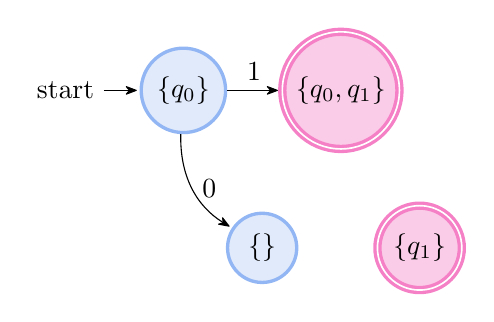
\begin{tikzpicture}[shorten >=1pt,node distance=2cm,on grid,>={Stealth[round]},
        every state/.style={draw=CornflowerBlue!70,fill=CornflowerBlue!20,very thick}, 
        accepting/.style={draw=magenta!50,fill=magenta!20, very thick,double},baseline=(current bounding box.center)]
        
        \node[state,initial] (q_0) {\(\{q_0\}\)}; 
        \node[state,accepting] (q_01) [right=of q_0] {\(\{q_0, q_1\}\)};
        \node[state] (emp) at (1, -2) {\(\{\}\)}; 
        \node[state,accepting] (q_1) [right=of emp] {\(\{q_1\}\)};

        \path[->] (q_0) edge node[above] {\(1\)} (q_01) 
                edge[bend right] node[right] {\(0\)} (emp); 
    \end{tikzpicture}
\end{center}
Remember that we need to do this for all the symbols in \(\Sigma\) so that this new machine is deterministic. 
Then, we just move on to the next state. 

For \(\{q_0, q_1\}\), we have two states instead of just one, so what we're going to do is take the union of both \(\delta(q_0, a)\) and \(\delta (q_1, a)\) for each symbol \(a\) in the alphabet. 
We already know that \(\delta(q_0,0) = \{\}\), and we have \(\delta(q_1,0) = \{q_1\}\). 
Thus, to get the new transition from \(\{q_0, q_1\}\) with symbol \(0\), we take the union of \(\{\}\) and \(\{q_1\}\), which is just \(\{q_1\}\). 
Likewise, we know that \(\delta(q_0, 1) = \{q_0, q_1\}\), and we have \(\delta(q_1, 1) = \{\}\), so our transition from \(\{q_0, q_1\}\) with symbol \(1\) will lead to \(\{\} \cup \{q_0, q_1\} = \{q_0, q_1\}\). 
\begin{center}
    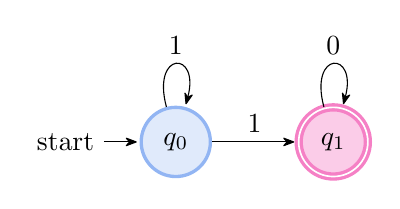
\begin{tikzpicture}[shorten >=1pt,node distance=2cm,on grid,>={Stealth[round]},
        every state/.style={draw=CornflowerBlue!70,fill=CornflowerBlue!20,very thick}, 
        accepting/.style={draw=magenta!50,fill=magenta!20, very thick,double},
        baseline=(current bounding box.center)]
        
        \node[state,initial] (q_0) {\(q_0\)}; 
        \node[state,accepting] (q_1) [right=of q_0] {\(q_1\)}; 

        \path[->] (q_0) edge [loop above] node {\(1\)} ()
                edge node[above] {\(1\)} (q_1) 
                (q_1) edge [loop above] node {\(0\)} (); 
    \end{tikzpicture}
    \hspace{20pt}
    \begin{tikzpicture}[shorten >=1pt,node distance=2cm,on grid,>={Stealth[round]},baseline=(current bounding box.center)]
        \path[dashed,->] (0,0) edge (1.5,0); 
    \end{tikzpicture}
    \hspace{20pt}
    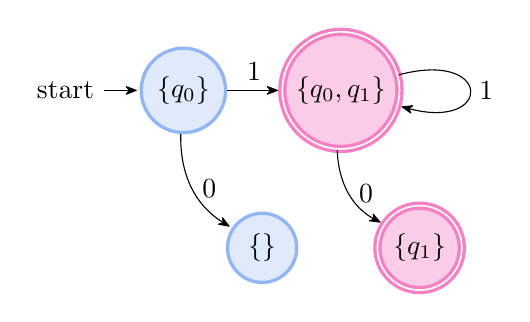
\begin{tikzpicture}[shorten >=1pt,node distance=2cm,on grid,>={Stealth[round]},
        every state/.style={draw=CornflowerBlue!70,fill=CornflowerBlue!20,very thick}, 
        accepting/.style={draw=magenta!50,fill=magenta!20, very thick,double},baseline=(current bounding box.center)]
        
        \node[state,initial] (q_0) {\(\{q_0\}\)}; 
        \node[state,accepting] (q_01) [right=of q_0] {\(\{q_0, q_1\}\)};
        \node[state] (emp) at (1, -2) {\(\{\}\)}; 
        \node[state,accepting] (q_1) [right=of emp] {\(\{q_1\}\)};

        \path[->] (q_0) edge node[above] {\(1\)} (q_01) 
                edge[bend right] node[right] {\(0\)} (emp)
                (q_01) edge[bend right] node[right] {\(0\)} (q_1) 
                edge[loop right] node[right] {\(1\)} (); 
    \end{tikzpicture}
\end{center}
Finally, I'll leave it as an exercise to see that we have the following transitions for \(\{q_1\}\): \[\{q_1\} \overset{0}{\to} \{q_1\}~~\text{and}~~\{q_1\} \overset{1}{\to} \{\}.\] 
For the state containing the empty set, it's pretty intuitive to see that it will be a trap state, as there are no transitions in the original machine from the empty set, so there are likewise no possible transitions. 
This gives us our final DFA:\begin{center}
    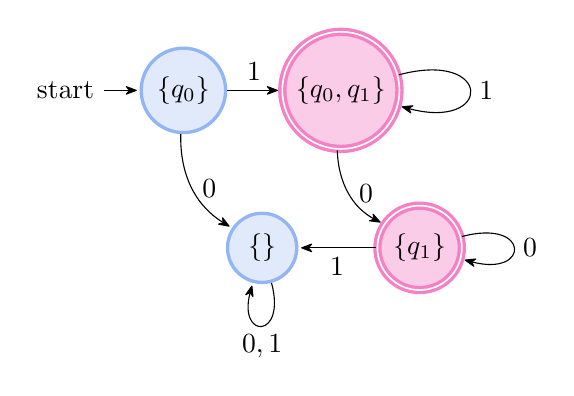
\begin{tikzpicture}[shorten >=1pt,node distance=2cm,on grid,>={Stealth[round]},
        every state/.style={draw=CornflowerBlue!70,fill=CornflowerBlue!20,very thick}, 
        accepting/.style={draw=magenta!50,fill=magenta!20, very thick,double},baseline=(current bounding box.center)]
        
        \node[state,initial] (q_0) {\(\{q_0\}\)}; 
        \node[state,accepting] (q_01) [right=of q_0] {\(\{q_0, q_1\}\)};
        \node[state] (emp) at (1, -2) {\(\{\}\)}; 
        \node[state,accepting] (q_1) [right=of emp] {\(\{q_1\}\)};

        \path[->] (q_0) edge node[above] {\(1\)} (q_01) 
                edge[bend right] node[right] {\(0\)} (emp)
                (q_01) edge[bend right] node[right] {\(0\)} (q_1) 
                edge[loop right] node[right] {\(1\)} ()
                (q_1) edge[loop right] node[right] {\(0\)} ()
                edge node[below] {\(1\)} (emp)
                (emp) edge[loop below] node[below] {\(0,1\)} (); 
    \end{tikzpicture}
\end{center}
One way we can check is to see if our construction is correct is to see if both machines compute the same language. 
It's easy to see that the language of our original machine is \(\lang = \{1^m 0^n \mid m > 0, n\ge 0\}\), and a quick inspection shows that the DFA computes the same language. 
\endex%

To prove Theorem~\ref{theo:equiv-nfa-dfa} we just have to generalize this argument to any arbitrary NFA, and show that the language that the new DFA computes is the same language as the original NFA. 

\begin{proof}
    %TO-DO
\end{proof}

\section{Regular expressions}\label{sec:regex}

Now, we switch gears to something entirely different. 
This whole time, we've been using semantics to define the regular languages. 
That is to say, we've been looking at DFAs and the process of computation itself in order to delineate which languages are regular and which languages aren't. 
We've also been using DFAs to study and understand regular languages. 
But what if we never had to look ``under the hood''---what if we had a characterization of the regular languages that never even referred to a DFA? 

This is precisely what the \emph{regular expressions} are for. 
They are a machine independent way of defining the regular languages. 
Think of the DFA as the underlying processor of your computer, and the regular expressions as a programming language. 
We \textit{could} talk about all we need to do with a computer entirely in terms of the inner workings of the processor, and all the voltage changes that happen in order to compute something, but we don't, because that would be ridiculous. 
Instead, we abstract away the unimportant details, and try to find away to identify what really matters in terms of the computation we're dealing with---which is precisely what we do when we write in programming languages. 


\section{The pumping lemma} 

There's a certain characteristic of DFAs that we've been using without really realizing how important it is. 
Consider any ``meaningful'' regular language (meaningful in the sense that it isn't just a finite list of strings). 
A lot of the languages we've been dealing with have had an infinite amount of possible strings. 
Even if the strings themselves have finite length, there's infinitely many of them to accept---sometimes several for every natural number---but our DFAs only have finitely many states. 
If we think about it, this is because our DFAs often have \textit{loops} that keep them stuck in the same few states. 

We often refer to the process of repeating \(v\) as ``pumping'' it, hence the name of the following theorem. 
\begin{theorem}[Pumping lemma for regular languages]
    For every regular language \(\lang\), there exists a positive integer \(n\) for which every string \(z\in\lang\), with \(|z| \ge n\) can be broken up into \(z = uvw\), where\vspace{-10pt}\begin{enumerate}\renewcommand{\labelenumi}{\colorbox{Periwinkle!20}{\textbf{\arabic{enumi}}}}
        \item \(|uv| \le n\); 
        \item \(|v| > 1\); and 
        \item for every integer \(i \ge 0\), \(z' = u v^i w\) is still a member of \(\lang\). 
    \end{enumerate}
\end{theorem}

\end{document}